
\begin{figure}
\begin{center}
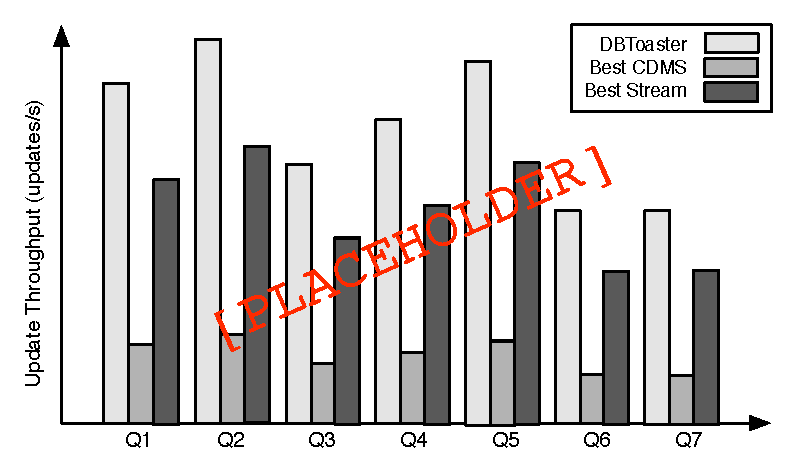
\includegraphics[width=3in]{../graphics-tmp/placeholder_bakeoff}
\end{center}
\label{fig:experiments:bakeoff}
\caption{Comparison of \dbtoaster\ with the best performing dbms and stream processor on each of the test queries}
\end{figure}

We now analyze the performance of \dbtoaster.  As in Section \ref{sec:dbfail}, experiments are run on \todo{insert hardware configuration here}.  Our analysis uses the queries from Examples \ref{ex:dbfail:stock}(PRICESPREAD),  \ref{ex:dbfail:tpch}(SHIPPING), and \ref{ex:dbfail:network}(NETFAIL), Queries numbers 3, 11, 17, 18, and 22 from the TPC-H\cite{tpch} benchmark, and the VWAP query presented in \cite{kennedy-ahmad-koch-cidr:11}.  Note that DBToaster is able to take advantage of the TPC-H benchmark's append-only nature: The SHIPPING and the TPC-H queries are compiled without deletion triggers.

First, we present \dbtoaster\ in comparison to existing techniques.  Figure \ref{fig:experiments:bakeoff} is a side-by-side comparison of \dbtoaster\ and the best performing (selected per-query) database management system and stream processor from Section \ref{sec:dbfail}.  The database management systems were tested using incremental view maintenance, and the stream processors were tested using the incremental implementation of each query.  \todo{ON +DATA:} \dbtoaster 's performance is superior to both types of system. 

\subsection{Throughput}
The three primary advantages of \dbtoaster\ are: (1) a recursive compilation algorithm, (2) set-based functional optimizations of the resulting program, and (3) compilation to machine code.  We now analyze each of these by isolating each optimization in turn within the \dbtoaster\ compiler.

\tinysection{Recursive Compilation}
\begin{figure}
\begin{center}
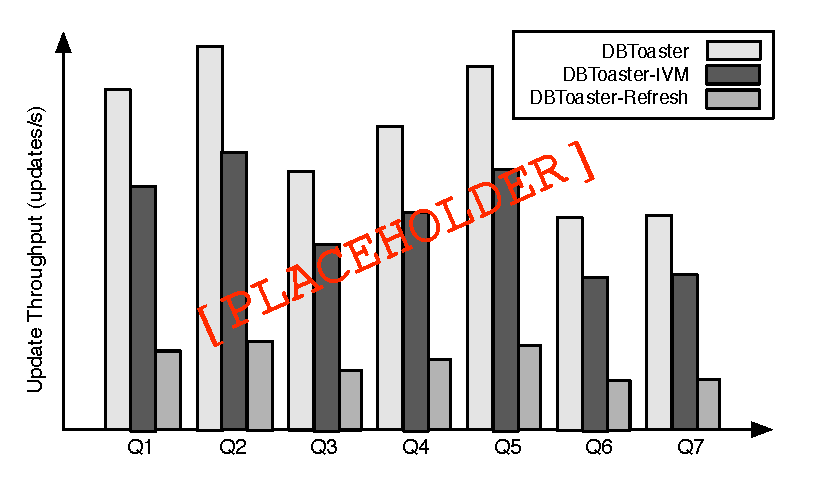
\includegraphics[width=3in]{../graphics-tmp/placeholder_throughput_all}
\end{center}
\label{fig:experiments:throughput_depth}
\caption{Comparison of \dbtoaster\ invoked with full recursive compilation, and with varying levels of depth restricted compilation.}
\end{figure}

\begin{figure}
\begin{center}
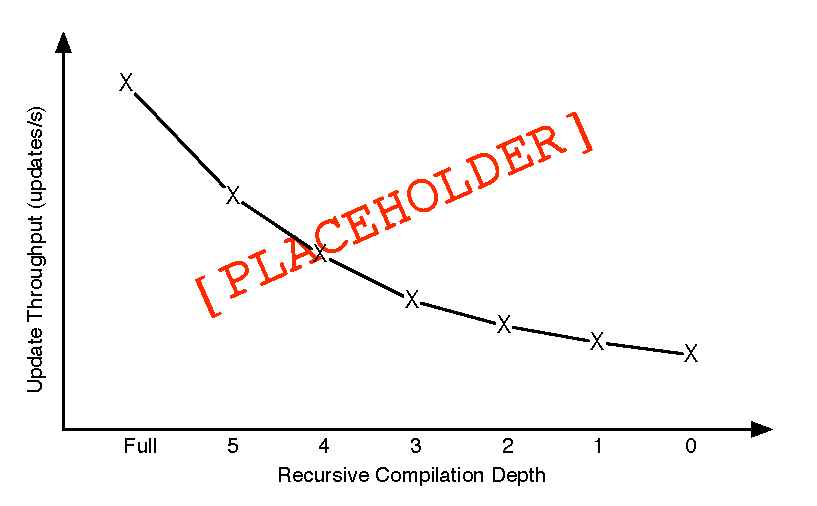
\includegraphics[width=3in]{../graphics-tmp/placeholder_throughput_ssb4}
\end{center}
\label{fig:experiments:throughput_depth_ssb4}
\caption{Varying \dbtoaster 's compile depth on a high-join width query.}
\end{figure}

\dbtoaster 's recursive compilation algorithm can be terminated early after reaching a predefined depth.  Delta queries below this depth are not materialized and incrementally maintained, but rather computed online from the base relation when they are needed.  Terminating at a depth of 0 corresponds to naive-re-evaluation of the query on every update, and terminating at a depth of 1 corresponds to Incremental View Maintenance.  Results of this early termination are presented in Figure \ref{fig:experiments:throughput_depth}.  

Of all of these queries, the SHIPPING query is an extremely wide (7-way) join, and provides an interesting insight into the benefits of the recursive compilation algorithm.  With each recursion, the compiler effectively removes one table from consideration -- the maximum recursion depth is the join width.  Figure \ref{fig:experiments:throughput_depth_ssb4} shows this, by relating query performance to the recursive depth.

\tinysection{Functional Optimizations}
\begin{figure}
\begin{center}
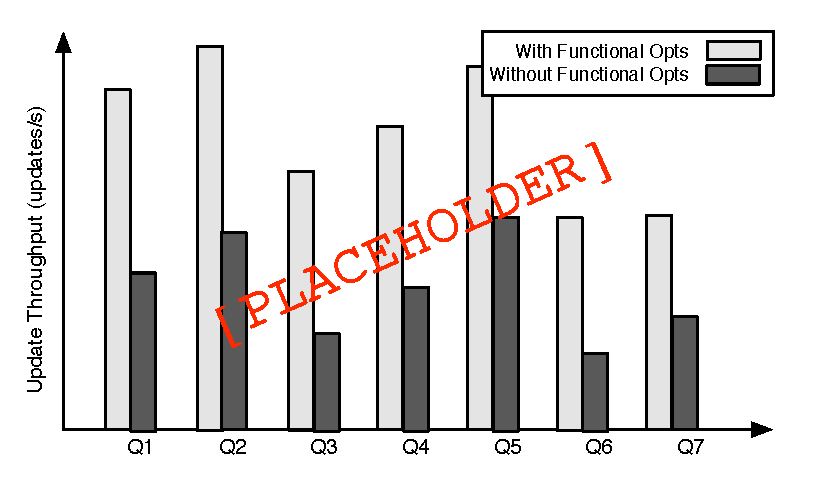
\includegraphics[width=3in]{../graphics-tmp/placeholder_throughput_k3opt}
\end{center}
\label{fig:experiments:throughput_functional}
\caption{Comparison of \dbtoaster\ invoked with and without functional optimizations.}
\end{figure}
Figure \ref{fig:experiments:throughput_functional} shows a comparison of \dbtoaster\ with the functional optimizations discussed in Section \ref{sec:functional} turned on to it with them turned off.  \todo{do we need finer granularity analysis here?}

\tinysection{Compilation}
\begin{figure}
\begin{center}
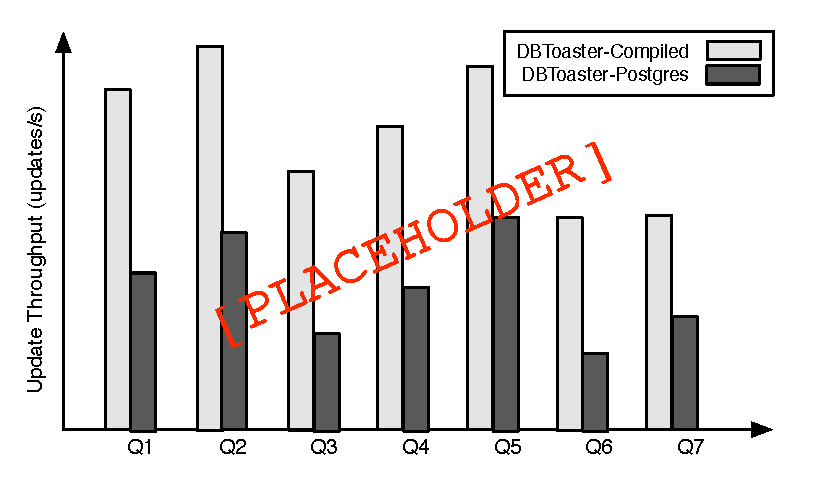
\includegraphics[width=3in]{../graphics-tmp/placeholder_throughput_compile}
\end{center}
\label{fig:experiments:throughput_compile}
\caption{Comparison of \dbtoaster\ invoked with compilation to C++ and with compilation to Postgres triggers.}
\end{figure}
Finally, we compare the benefits of compiling directly to machine code by using \dbtoaster\ to compile a trigger program in pl/pgSQL that is equivalent to the program it would further compile into machine code.  The resulting trigger program is run on a Postgres database and compared to the equivalent machine code.  The results of this comparison are shown in Figure \ref{fig:experiments:throughput_compile}.

\subsection{Costs}
\begin{figure}
\begin{center}
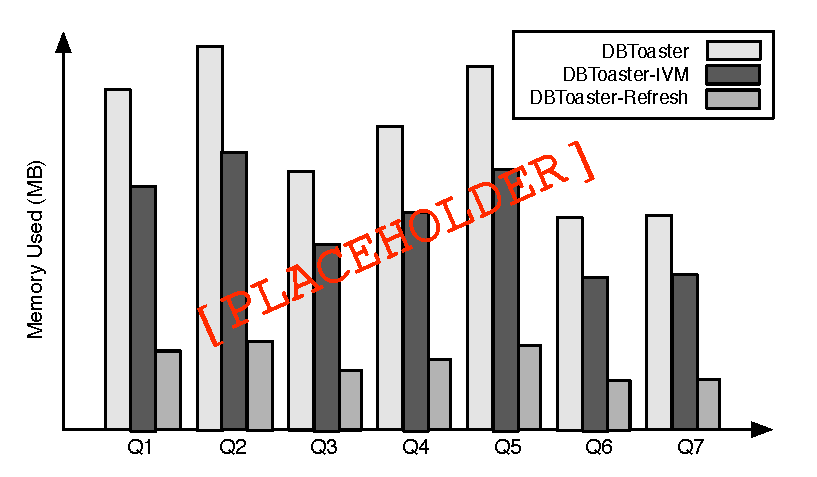
\includegraphics[width=3in]{../graphics-tmp/placeholder_memory_all}
\end{center}
\label{fig:experiments:memory}
\caption{Peak memory used by \dbtoaster\ for full recursive compilation and with varying levels of depth restricted compilation.}
\end{figure}

\begin{figure}
\begin{center}
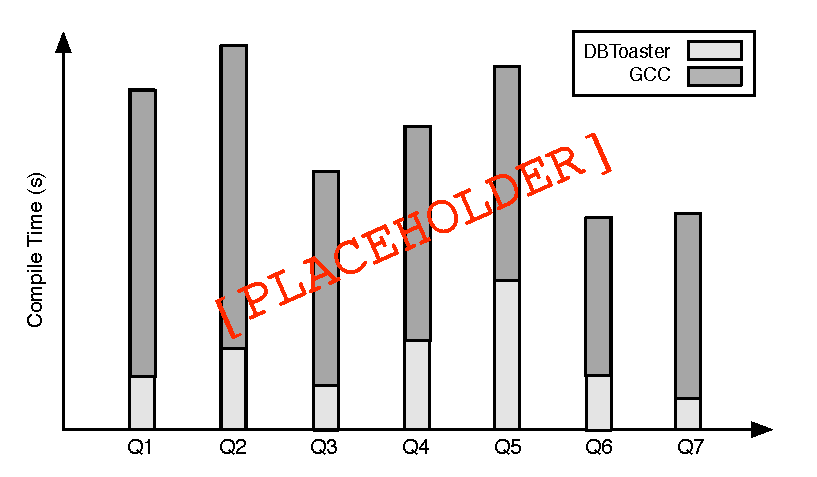
\includegraphics[width=3in]{../graphics-tmp/placeholder_compile_all}
\end{center}
\label{fig:experiments:compile}
\caption{Time taken by the \dbtoaster\ compiler to compile each of the test queries.}
\end{figure}

The throughput improvements of \dbtoaster\ come at the cost of increased memory usage and compile times.  Figure \ref{fig:experiments:memory} shows the peak memory used by the \dbtoaster\ runtime to store persistent state for each of the queries in the workload.  The peak memory usage for compilation terminated at recursive depths of 0 and 1 are also shown.  As Figure \ref{fig:experiments:throughput_depth} shows, the reduction in memory usage corresponds directly to lower update throughputs.

Figure \ref{fig:experiments:compile} shows the amount of time taken to compile each query.  Although these compile times are not suitable for realtime querying, they are acceptable for long-running monitoring applications.  Also note that the dominant cost of compilation in each case is \dbtoaster 's invocation of GCC to translate from C++ to machine code.  This cost can be eliminated by compiling directly to machine code or an intermediate bytecode such as LLVM \cite{llvm}.


